\documentclass[a4paper,11pt]{article}

% Encodage et langue
\usepackage[utf8]{inputenc}
\usepackage[T1]{fontenc}
\usepackage[french]{babel}

% Marges
\usepackage[a4paper,margin=2.5cm]{geometry}

% Gestion des citations
\usepackage[backend=biber,style=authoryear]{biblatex}
\addbibresource{bibliography/references.bib}

% Packages supplémentaires
\usepackage{graphicx} % Pour les images
\usepackage{amsmath, amssymb} % Pour les maths
\usepackage{hyperref} % Pour les liens hypertextes
\usepackage{setspace} % Pour ajuster l'interligne
\usepackage{titlesec} % Pour personnaliser les sections
\usepackage{subcaption} % Pour les sous-figures

% Configuration des liens
\hypersetup{
    colorlinks=true,
    linkcolor=blue,
    citecolor=blue,
    urlcolor=blue,
}

% Personnalisation des sections
\titleformat{\chapter}[hang]
{\normalfont\huge\bfseries}{\thechapter.}{1em}{}

\begin{document}

% Page de titre
\title{A Regularized Wasserstein Framework for Graph Kernels}
\author{Grégoire Béchade}
\date{17/01/2025}
\maketitle

\section{Abstract}

% Introduction
\section{Introduction}

The authors of this paper aim to develop a Wasserstein distance between graphs, in order to perform graph classification. 





\section{Theoretical Background}

The objective of the paper is to be able to define a optimal transport plan between two graphs. 
But, optimal transport enables to have access to a mapping between probability distrivutions. 
The first issue is to transform a graph into a probability distribution.\\[0.5cm]
\textbf{Notations:} \\
Let $G=(V, E)$ a non-oriented graph with $V$ the set of vertices and $E$ the set of edges.
We note $n$ the number of vertices and $m$ the number of edges.
We consider $\xi_f : V \rightarrow \mathbb{R}^m$ a feature embedding function (TODO ADD REF), and $\xi_s : V \rightarrow \mathbb{R}^k$ a structure embedding function TODO ADD REF.\\
We can therefore associate to each vertex of the graph a single point in $\mathbb{R}^m \times \mathbb{R}^k$, and therefore a probability distribution on $\mathbb{R}^m \times \mathbb{R}^k$ : $p = \sum_{i=0}^{n} \mu_i \delta(\xi_f(v_i), \xi_s(v_i))$, with $\mu_i$ the weight of the vertex $v_i$ (set to $\frac{1}{n}$ if none is provided).\\


We are now equipped with a function that takes as an input a graph and outputs a probability distribution.
We can easily define a distance between those two graphs, by computing the Wasserstein distance between the two associated probability distributions and solve the Kantorovich problem. 
However, the authors introduce two regularization terms and a clever cost matrix in the Wasserstein distance to take into account feature and structure similarity between graphs. \\[0.5cm]

\textbf{Problem formulation:} \\
Let $G_1$ and $G_2$ two graphs, and $\mu1$ and $\nu$ their associated probability distributions.
The authors define the RW discrepancy between of these two graphs as : \\

$RW(\mu, \nu) = \underset{\gamma \in \pi(\mu, \nu)}{\operatorname{min}} {\left\langle \gamma , C^V \right\rangle}_F   + \beta_1 LW(\mu, \nu)  +\beta_1 GW(\mu, \nu) $\\

We will explain the different terms of this equation in the following sections.

\subsection{$C^V$ : a cost function to reflect feature similarity}
\label{CV}
We consider a graph $G=(V, E)$ and a graph signal $(x_i)_{i \in \{1, ..., |V| \} } \in \mathbb{R}^m$, which is just a function on the vertices of the graph. 
This signal can for instance be the value of a physical quantity in a graph of sensors, or the number of followers of a user in a social network.
TODO ADD REF TO MLTS. 
We can therefore associate to a graph a signal matrix $X \in \mathbb{R}^{n \times m}$ (with $n$ the number of nodes and $m$ the space in which those features leave).

The local variation matrix of $G$ is defined as : $\Delta(X) = | X - \frac{1}{\lambda_{max}(L)} L^j X  |$, with $L$ the graph Laplacian and $\lambda_{max}(L)$ its largest eigenvalue.
The intuition behind this matrix is to measure the variation of the signal between two nodes of the graph.
Considering a node $v_i$, its feature $x_i \in \mathbb{R}^m$ and the corresponding local variation $\Delta(x_i) \in \mathbb{R}^m$, the authors define the feature embedding function as $\xi_f(v_i) = [x_i, \Delta(x_i)] \in \mathbb{R}^{2m}$.

Finally, the feature similarity matrix, that will later be used as a cost matrix in the Wasserstein distance, is defined as  matrix in $\mathbb{R}^{n_1 \times n_2}$: $C^V(i,j) = d_f(a_i, a_j) $, with $d_f$ a distance function, which will be the $L_2$ distance in the paper.

This cost function means that it costs many to match nodes with different features, in terms of values but also of variations. 
The intuition behind this is that we want to take into account the behaviour of the graph signal when assessing the difference between two graphs.


\subsection{LW : a regularization term to preserve neighbourhood similarity}
\label{LW}
The first regularization term is the Local Barycentric Wasserstein Distance (LW). 
This term enables to neighbourghood similarity, by solving once again a Wasserstein distance problem, but with a different cost matrix.
The cost matrix of this distance is $C^N(i,j) = (d_s(e_i, e_j))_{i,j} \in \mathbb{R}^{n_1 \times n_2}$, with $e_i$ and $e_j$ the node embeddings of the nodes $i$ and $j$ from the two graphs, and $d_s$ a distance function, which will be set as the hammer distance. 
However, the hammer distance is not defined for continuous variables, and the authors did not explai how they managed to compute it.
A extension of hammer distance to continuous variables was found in \cite{labib2019hamming}, and might be the adaptation used? 
This cost matrix reflects the idea that this term preserves the similarity between connected nodes in the transport plan: it costs lots to associate a vertex from $G_1$ to a vertex of $G_2$ if their embeddings are far away.\\
This cost matrix enables to associate nodes only of their embeddings are close, which seems intuitive: two similar nodes whould be associated together with a small cost.
However, nothing enables the user to be sure that two connected nodes in $G_1$ will end up close in $G_2$, after the transportation. 
That is why the authors introduced a regularization term to enforce this property.

Formally, let us define $ \hat{e}_i^\mu = \frac{\sum_{j=1}^{n_2} \gamma(i,j)e_j^{\nu}}{\sum_{j=1}^{n_2} \gamma(i,j)}$. 
This vector is the barycenter of the embeddings of the nodes of $G_2$ that are connected to the node $i$ of $G_1$.
Then the source regularization term is defined as : \\
This source regularization term is minimized when two connected nodes of $G_1$ are sent by the transport plans to two groups of nodes whose barycenters are close.\\
The target regularization term can be defined in the same way, as : $\Omega_\nu(\gamma) = \frac{1}{n_2^2} \sum_{i,j} b_{i,j} \left\lVert \hat{e}_i^\nu - \hat{e}_j^\nu\right\rVert ^2 $, with $b_{i,j}$ the adjacency matrix of $G_2$.

We can now define the regularization term of the LW distance between to graphs as : 
\\ $\Theta_\omega(\gamma) = \lambda_\mu \Omega_\mu(\gamma) + \lambda_\nu \Omega_\nu(\gamma) + \frac{\rho}{2} \left\lVert \gamma \right\rVert _F^2 $\\

Finally, we have : \\

$LW(\mu, \nu) = \underset{\gamma \in \pi(\mu, \nu)}{\operatorname{min}} {\left\langle \gamma , C^N \right\rangle}_F + \Theta_\omega(\gamma)$\\


This distance preserves a proximity between nodes connectes by the transport plan and between nodes connected in the graphs.
% Le barycentre de la ou deux points envoient de la masse doit être proche si ces deux points sont connectés. 
% Le coût est élevé si duex noeuds connectés sur un graphe sont envoyés à des endroits distants. 


A result from the paper is that this distance is strongly convex and smooth with respect to $\gamma$, which provides guarantees for the convergence of the algorithm.\\


\subsection{GW : a regularization term to preserve pairwise similarity}
\label{GW}
A last term is introduced to preserve the pairwise similarity between matrixes. 
As done above, a cost matrix $C^P$ is defined as : $C^P(i,j) = d_s(e_i, e_j)$, with $d_s$ a distance function and $e_i$, $e_j$ the node embeddings of the nodes $i$ and $j$ of the considered graph. 
A $C^P$ matrix is defined for each pair of graphs, and the pairwise similarity between $G_1$ and $G_2$ is defined as the following 4-dimensional tensor (I noted taht this approach was also found in \cite{titouan2019optimal}) : 

$L_2(C_1^P(i,j), C_2^P(k,l)) = \left\lvert C_1^P(i,j) - C_2^P(k,l) \right\rvert ^2 $. \\

The Gromov-Wasserstein distance is then defined as : \\

$GW(\mu, \nu) = \underset{\gamma \in \pi(\mu, \nu)}{\operatorname{min}} {\left\langle \gamma , L_2(C_1^P, C_2^P) \otimes \gamma \right\rangle}_F - \lambda_g \Theta_g(\gamma)$, with $\Theta_g(\gamma) $ the Kulback Liebler divergence between $\gamma$ and a prior distribution named $\gamma '$ in the paper.

The authors note that the Gromov Wasserstein distance is not convex, but the introduction of the regularization term enables to have better convergence properties. \\[2cm]

Finally, we have explained all the terms of the RW discrepancy, which computes an optimal transport plan between two "clever" probability distributions representing the graphs, while preserving neighbourghood similarity (see \ref{LW}), pairwise similarity (see \ref{GW}) and feature similarity (see \ref{CV}).
However, solving the problem is very hard, and the authors propose an algorithm to solve it, which is detailed in the next section.


\subsection{An algorithm to solve the problem}

In the paper, an algorithm named Sinkhorn Conditionnal Gradient is introduced to find the transport plan between the two graphs $G_1$ and $G_2$. 
The idea of the algorithm is the following: at each step, the gradient of the loss function is computed $(\nabla H(\gamma))$, and a direction of descent is determined as the transport plan that minimizes the OT transport between $\mu$, $\nu$, with $\nabla H (\gamma)$ as the cost function, with Sinkhorn algorithm.
The step size is then determined through a grid-search, and the algorithm stops when the convergence criterion is met, or the maximum number of iterations is reached.

Corrolary 1 of the paper states that it takes $O(\frac{1}{\epsilon^2})$ iterations to find a solution whose sub-optimality gap is below $\epsilon$. 

This algorithm has a complexity of $O(t(n^3 + kn^2 ))$ with $t$ the number of iterations, $n = max(n_1, n_2)$ the number of nodes in the largest graph, and $k$ the dimension of the embeddings of the nodes. 
However, in my experiences, I have noticed that the computational time was multiplied by a factor 9 when the number of nodes was multiplied by 3, so the dominant term might be the squared one. 
This complexity is therefore similar to the one of the Sinkhorn algorithm, which has a complexity of $O(T \times n^2)$. 
However, with different datasets, the complexity might be in $n^3$ and the computational time might be very high.

\subsection{Some concepts}

Some key points of the method are not explained in the paper and lead to some research. 
They are detailed in the following sections.

\subsubsection{Kernel classification}

\textbf{Kernel method: } \\

The main objective of the paper is to be able to determine a clever distance between graphs in order to perform efficient classification of those graphs through kernel methods. 
The idea of kernel methods is that we like to have linearly separable sata when it comes to classification. 
very simple algorithms such as SVM can then be used to classify data. 
however, it is very common to have non linear separable data. 
The idea of kernel methods is to define a function $\phi$ that maps the data into a higher dimesional space, in which they are then linearly separable. 
The SVM algorithms then finds an hyperplan that separates the two classes by maximizing the margin between the two classes.
An hyperplan is defined by its normal vector $w$ and its bias $w_0$.
The points on the hyperplan are the one following this equation : $w^T \phi(x) + w_0 = 0$.
The points on a side of the hyperplan are the ones for which $w^T \phi(x) + w_0 > 0$, and on the other side the inverse inequality. 
A separator hyperplan is the the one that separates the two classes : $\forall k, sgn(y_k) \times (w^T\phi(x_k)+w_0) \geq 0 $. 
The optimal hyperplan is the determined by maximizing the margin between the two classes:  \\

$w_{opt} =  \underset{w, \forall k y_k(w^Tw_k+w_0 \geq 1)}{\operatorname{min}}  \frac{1}{2} \left\lVert w\right\rVert^2 $\\[0.2cm]

The dual form of this optimization problem is : \\

\begin{align}
     & \underset{\alpha_k \geq 0 \sum_{k=1}^{p} \alpha_k y_k = 0 }{ max }   \sum_{k=1}^{p} \alpha_k -\frac{1}{2}  \sum_{i,j} \alpha_i \alpha_j y_i y_j \phi(x_i)^T \phi(x_j) \\
    = & \underset{\alpha \geq 0, \alpha^T y = 0 }{max}  \alpha^T e - \frac{1}{2}Tr(K(Y\alpha)(Y \alpha)^T) 
\end{align}
(with the notations from \cite{lanckriet2004learning}).\\[1cm]

\textbf{Kernel trick: } \\



However, this method can be very computationally expensive, as the dimension of the space in which the data is mapped can be very high.
The kernel trick introduces a kernel function $K(x, x') = \phi(x)^T \phi(x')$ that enables to compute the dot product in the higher dimensional space without computing the mapping $\phi$.
Indeed, with the previous notations, the separator hyperplan can be written as : $\{ x \in \mathcal{X}, s.t. w^T \phi(x) + w_0 =0  \} $, which can be re-written as $\{ x \in \mathcal{X}, s.t.  K(w, x) + w_0 = 0 \}$. 
This trick enables to prevent to compute the mapping $\phi$. 
According to Mercer's theorem (\cite{mercer1909xvi}), a function $K$ is a valid kernel if and only if the matrix $K$ is positive semi-definite, which is not the case in the article studied. 
To overcome this issue, the authors decide to treat their undefinite kernel as the noisy observation of a true kernel. 
The idea is to solve the problem for a semi definite positive kernel ($K$) that is very close to the one actually used ($K_0$).
With the same notations as \cite{lanckriet2004learning}, the problem becomes : \\

$  \underset{K \succeq 0 }{min } \underset{\alpha^T y = 0, 0 \leq \alpha \leq C}{max}  \alpha^T e - \frac{1}{2}  Tr(K(Y \alpha) (Y \alpha)^T) + \rho \left\lVert K - K_0\right\rVert _F ^2 $\\[0.3cm]
The idea is from \cite{luss2007support}, who introduces a penalty term instead of looking for a very close semi definite positive kernel.\\

\begin{figure}[h]
    \centering
    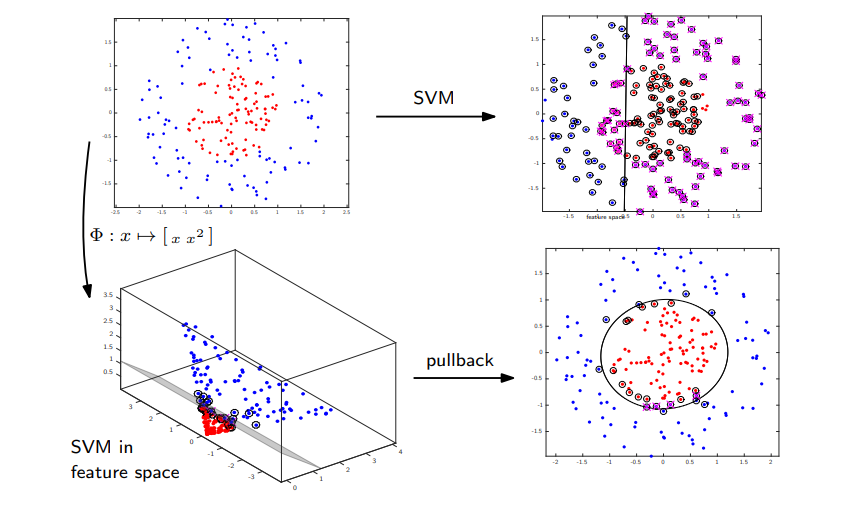
\includegraphics[width=0.5\textwidth]{figures/kernel_trick.png}
    \caption{Illustration of the kernel trick, from \cite{oudot2022cpp}}
\end{figure}

\textbf{Example with the Gaussian kernel: } \\

A common kernel is the gaussian kernel. 
Let $x$ and $x'$ two points in $\mathbb{R}^d$.
The gaussian kernel is defined as : $K(x, x') = exp(-\frac{\left\lVert x - x' \right\rVert ^2}{2\sigma^2})$.\\
$K(x, x') = e^{-\frac{\left\lVert x \right\rVert ^2}{2\sigma^2}} \times e^{-\frac{\left\lVert x' \right\rVert ^2}{2\sigma^2}} \times e^{ \frac{x^T x'}{\sigma^2}}$.\\
However, $e^{\frac{x^T x'}{\sigma^2}} = \sum_{k=0}^{\infty} \frac{1}{k!} \left( \frac{x^T x'}{\sigma^2} \right)^k$, which can be expressed as a scalar product. 


\subsubsection{Heat kernel random walk}

As discussed above, a key step of the method is to define an embedding function that takes as an input a node and outputs a vector in $\mathbb{R}^m$.
Two embedding functions are used: one for the features on the node ($\xi_f$) and one for the structure of the node ($\xi_s$).
The idea of the heat kernel random walk is to learn for each graphe an embedding function. 
The method is explained in \cite{abu2018watch}. 
The idea is to randomly select a node of the graph ($v_0$), and then to randomly select a neighbour of this node($v_1$), and continue until a certain number of steps is reached.
This leads to a chain of linked nodes $v_0, v_1, ..., v_k$.
The embedding of a node $v_i$ is then moved closer to the embedding of the following nodes $ v_{i+1}, \dots, v_{i+C} $, with $C$ a context parameter. 


\section{Numerical Experiments}

As the code was available \href{https://github.com/wokas36/RWK}{here}, I decided to test it on a simple classification task to assess the performance of the method and the influence of some parameters. 

\subsection{Data}

I decided to perform a very simple classification task on nearest neighbourghs graphs. 
The graphs were generated with the following methodology : \\
\begin{itemize}
    \item Sample uniformly \textit{n=15} points in $[-1, 1]^2$. 
    \item Connect each point to its k nearest neighbours.
    \item Set the coordinates of the point as the node value. \\
\end{itemize}

The two classes of graphs correspond to values of $k$ equal to \textit{2} and \textit{3}.

I have then generated a training set of 400 graphs, containing 200 graphs of each class, and a test set of 100 graphs, containing 50 graphs of each class.\\

% sub figure pour les deux classes de graphes : 
\begin{figure}[h]
    \centering
    \begin{subfigure}{0.4\textwidth}
        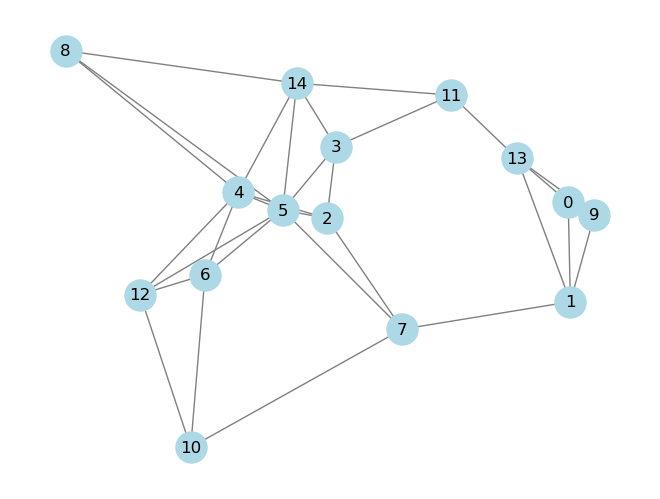
\includegraphics[width=\textwidth]{figures/graph_k3.png}
        \caption{Example of a graph with k = 2 }
    \end{subfigure}
    \begin{subfigure}{0.4\textwidth}
        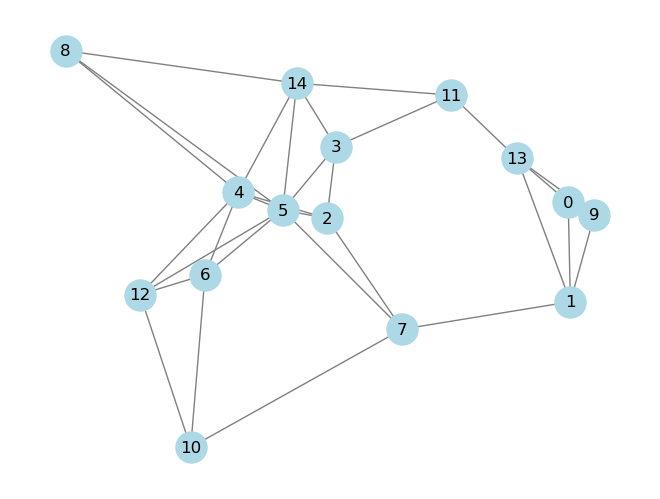
\includegraphics[width=\textwidth]{figures/graph_k3.png}
        \caption{Example of a graph with k = 3}
    \end{subfigure}
    \caption{Example of two graphs of each class}
\end{figure} 


\textbf{Some insights on the data: }\\

The 200 2-nn graphs contain TODO ADD NUMBER edges in average. 
The 200 3-nn graphs contain TODO ADD NUMBER edges in average.
See Fig. \ref{fig:hist_edges} for more details. 

56.5 \% of the 2nn graphs are connected, and 90.0 \% of the 3nn graphs are connected.


\begin{figure}
    \centering
    \begin{subfigure}{0.4\textwidth}
        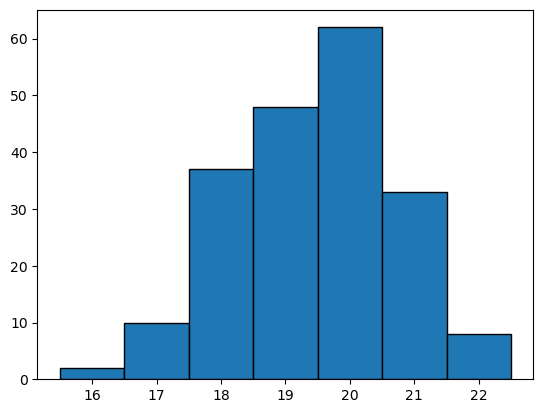
\includegraphics[width=\textwidth]{figures/hist_2_nn.png}
        \caption{Distribution of the number of edges in the graphs with k = 2}
    \end{subfigure}
    \begin{subfigure}{0.4\textwidth}
        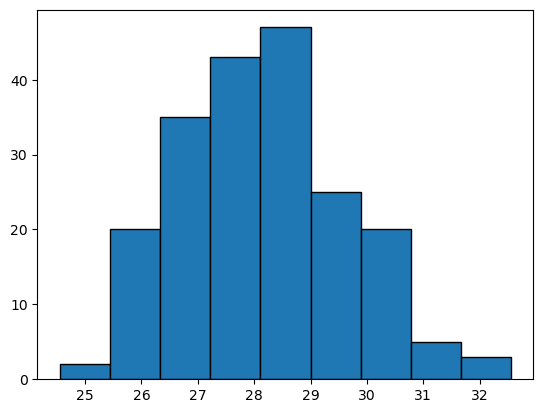
\includegraphics[width=\textwidth]{figures/hist_3_nn.png}
        \caption{Distribution of the number of edges in the graphs with k = 3}
    \end{subfigure}
    \caption{Number of edges in the train set}
    \label{fig:hist_edges}
\end{figure}


\subsection{Methodology}

The SVC classifier implemented in the paper was used to classify the graphs. 
It was trained on the training set and tested on the test set.
The performances was evaluated through accuracy and F1 score.
I also decided to study the impact of the differnt terms by setting some regularization terms to 0 and by making some vary along different values. 
The computational time and the performances in term of F1-scorr and accuracy was were then compared. 

Two baselines model were also tested: the default random forest classifier from sklearn, and a SVM classifier with a gaussian kernel.





\subsection{Results}

\section{Conclusion}

critique : code ne marche pas, très long pour des résultats pas si fou 
petites erreurs : " two strongly convex terms " ben boyons... on me prend pour un jambon.

\section{Connection with the course}

First, a question that arises in the paper is to find the optimal transport plan between two graphs, which are ambedded as points in $\mathbb{R}^m \times \mathbb{R}^k$.
This problem is an optimal transport between two sums of a different amount of diracs in very high dimension. 
It therefore corresponds to the Kantorovich problem with discrete distributions, that was studied in the course 2. 
However, the authors have a differnet approach than the one studied in course to solve this problem. 
Instead of adding an entropic regularization that makes the problem strictly convex, they introduce two regularization terms that enable to preserve the structure of the graphs, but make the computations harder. 



The whole problem of the paper is to solve an optimal transport between two probability distributions, with a penalty adapted to the nature of the data. 
It has a clear link with the course 4, that presents another algorithm to solve the optimal transport problem: the Sinkhorn algorithm.
In the course, the penalty was the Shannon entropy of the transport plan, while the two penalties introduced in the paper are the local barycentric and the global connectivity penalties.
The difference with the course is that the Shannon penalty makes the problem strictly convex, while despite the fact that the gloabl barycentric penalty is strongly convex with respect to $\gamma$, the Gromo-Wasserstein distance is not convex, and therefore leads to a more complex optimization problem.
Therefore, the authors managed to prove that the algorith converges toward a stationary point, there is no guarantees on the convergence to the global minimum.
On the contrary, the Sinkhorn algorithm consists in iterations of a contracting function, which has as a consequence that the algorithm converges. 


connection avec cours 4: régularisation intelligente. 
Par contre le problème n'est pas strictement convexe

lien avec sinkhorn, différences avec l'algo vu en cours. 


\newpage
\printbibliography

\end{document}